\documentclass[a4paper,12pt,twoside]{article}
\usepackage[left=1in,right=1in,top=1in,bottom=1in]{geometry}

\usepackage{xeCJK}
\setCJKmainfont{Songti TC}
\setCJKfamilyfont{kai}{Songti TC}
\newcommand{\kai}{\CJKfamily{kai}} % 用 \kai{使用楷書}

\usepackage{lmodern}
\usepackage{titling}
\usepackage{titlesec}
\usepackage{graphicx}
\usepackage{float}
\usepackage{amsmath, amsthm, amssymb, amsfonts, mathrsfs}
\usepackage{upgreek} % 直立的希臘字母

\usepackage[shortlabels]{enumitem}
\usepackage{setspace}
\renewcommand{\baselinestretch}{1.5}
\usepackage[colorlinks]{hyperref}
\usepackage{fancyvrb}
\usepackage{fancyhdr}
\usepackage{multicol}
\usepackage{caption}
\usepackage{listings}
\usepackage{bm}
\usepackage{bbm} % for \mathbbm{1} (indicator function)
\usepackage{centernot}
\usepackage{mdframed}
\usepackage{tikz}
\usetikzlibrary{patterns, arrows.meta, positioning}
\usepackage[nameinlink, capitalise]{cleveref}
\usepackage{diagbox}
\usepackage{booktabs}
\usepackage{multirow,array}
\usepackage{tabularx}
\usepackage{mathtools}
\usepackage{indentfirst} % 首段 indent
\setlength{\parindent}{2em}
\usepackage{cancel} % 數學式子畫線槓掉
\newcommand\mcancel[2][red]{\setbox0=\hbox{$#2$}%
\rlap{\raisebox{.45\ht0}{\textcolor{#1}{\rule{\wd0}{1pt}}}}#2}
\usepackage{datetime2}

\AtBeginDocument{%
 \setlength{\abovedisplayskip}{6pt}
 \setlength{\belowdisplayskip}{6pt}
 \setlength{\abovedisplayshortskip}{4pt}
 \setlength{\belowdisplayshortskip}{4pt}
}

\definecolor{codegreen}{rgb}{0,0.6,0}
\definecolor{codegray}{rgb}{0.5,0.5,0.5}
\definecolor{codepurple}{rgb}{0.58,0,0.82}
\definecolor{backcolour}{rgb}{0.95,0.95,0.92}

\lstdefinestyle{mystyle}{
 backgroundcolor=\color{backcolour},
 commentstyle=\color{codegreen},
 keywordstyle=\color{magenta},
 numberstyle=\tiny\color{codegray},
 stringstyle=\color{codepurple},
 basicstyle=\ttfamily\footnotesize,
 breakatwhitespace=false,
 breaklines=true,
 captionpos=b,
 keepspaces=true,
 numbers=left,
 numbersep=5pt,
 showspaces=false,
 showstringspaces=false,
 showtabs=false,
 tabsize=2
}
\lstset{style=mystyle}

\hypersetup{citecolor=blue, linkcolor=blue, urlcolor=blue}

\DeclareMathOperator{\supp}{supp}
\DeclareMathOperator{\skewness}{Skewness}
\DeclareMathOperator{\DU}{D-U}
\DeclareMathOperator{\CU}{C-U}
\DeclareMathOperator{\Geo}{Geo}
\DeclareMathOperator{\Pois}{Pois}
\DeclareMathOperator{\Gam}{Gam}
\DeclareMathOperator{\LN}{LogN}
\DeclareMathOperator{\cov}{Cov}
\DeclareMathOperator*{\argmax}{arg\,max}
\DeclareMathOperator*{\argmin}{arg\,min}
\DeclareMathOperator{\re}{Re}
\DeclareMathOperator{\im}{Im}

\newcommand{\N}{\mathbb{N}}
\newcommand{\Z}{\mathbb{Z}}
\newcommand{\Q}{\mathbb{Q}}
\newcommand{\R}{\mathbb{R}}
\newcommand{\C}{\mathbb{C}}
\newcommand{\G}{\mathcal{G}}
\newcommand{\mP}{\mathbb{P}}
\newcommand{\F}{\mathcal{F}}
\newcommand{\B}{\mathcal{B}}
\newcommand{\1}{\mathbbm{1}}
\newcommand{\Poi}{\text{Poi}}
\newcommand{\Var}{\text{Var}}
\newcommand{\as}{\text{a.s.}}
\newcommand{\vect}[1]{\boldsymbol{\mathbf{#1}}}
\newcommand{\paren}[1]{\left({#1}\right)}
\newcommand{\brk}[1]{\left[{#1}\right]}
\newcommand{\curl}[1]{\left\{{#1}\right\}}
\renewcommand{\lambda}{\lambdaup}

\theoremstyle{definition} % 定理環境 style 改用正體
\newtheorem{theorem}{定理}
\newtheorem{definition}{定義}
\newtheorem*{definition*}{定義}
\newtheorem{example}{例子}
\newtheorem{exercise}{練習}
\newtheorem{corollary}{推論}
\newtheorem{property}{性質}
\newtheorem{prop}{命題}
\newtheorem{lemma}{引理}
\newtheorem{problem}{問題}
\newtheorem*{remark}{註}

\renewcommand{\figurename}{圖}
\renewcommand{\tablename}{表}

\DeclareMathOperator{\var}{Var}
\DeclareMathOperator{\corr}{corr}
\DeclareMathOperator{\rank}{rank}
\DeclareMathOperator{\MSE}{MSE}
\DeclareMathOperator{\SSE}{SSE}
\DeclareMathOperator{\SST}{SST}
\DeclareMathOperator{\SSR}{SSR}
\DeclareMathOperator{\sgn}{sign}
\DeclareMathOperator{\alt}{Alt}
\DeclareMathOperator{\adj}{adj}
\DeclareMathOperator{\curlOp}{curl}
\DeclareMathOperator{\spn}{span}
\DeclareMathOperator{\sse}{SSE}
\DeclareMathOperator{\tr}{tr}

\newcommand{\ep}{\varepsilon}
\newcommand{\p}{\partial}
\newcommand{\abs}[1]{\left|#1\right|}
\newcommand\norm[1]{\left\lVert#1\right\rVert}
\newcommand{\innerprod}[1]{\langle#1\rangle}
\newcommand{\ds}{\displaystyle}
\newcommand{\blank}{\rule[-1mm]{1.5cm}{0.1mm}}
\newcommand{\dint}{\displaystyle\int}
\renewcommand{\bar}{\overline}

\newtheoremstyle{remark}{}{}{}{}{\bfseries\sffamily}{.}{.5em}{#1}
\theoremstyle{remark}

\newtheorem*{remark*}{\textit{Remark}}
\newtheorem*{solution*}{解}

\AtEndEnvironment{solution*}{\hfill$\square$}
\newtheorem*{hint*}{Hint}


\newcommand{\redtext}[1]{{\color{red} #1}}
\newcommand{\bluetext}[1]{{\color{blue} #1}}

\fancypagestyle{firstpage}{
  \fancyhf{}
  \fancyhead[R]{\small《高中數學實驗教材》第 3 冊（自然組）}
  \fancyhead[L]{\small 第 1 章\quad 實際世界——幾何與代數}
  \fancyfoot[C]{\thepage}
}

\pagestyle{fancy}
\setlength{\headheight}{14pt}
\renewcommand{\headrulewidth}{0.5pt}
\renewcommand{\footrulewidth}{0pt}
\fancyhead{}
\fancyhead[LE]{\small 《高中數學實驗教材》第三冊（自然組）}
\fancyhead[RO]{\small 第一章\quad 實際世界——幾何與代數}
\fancyfoot[C]{\thepage}

\title{\LARGE\textbf{《高中數學實驗教材》第三冊（自然組）}\\[0.5em] \Large\textbf{第一章\quad 實際世界——幾何與代數}}
\author{\textbf{高中數學實驗教材編輯小組}\quad 編著}
\date{民國六十四年（1975）再版}

\begin{document}

\maketitle
\thispagestyle{firstpage}

% ==========================================
% 掃描檔勘誤、文字校訂與疑難處說明（依規則整理於目錄之前）
% ==========================================
\section*{【說明】第一章掃描檔勘誤、疑難處與文義校訂表}
\addcontentsline{toc}{section}{【說明】第一章掃描檔勘誤、疑難處與文義校訂表}
\label{sec:errata_notes_b3_ch1}

本章依據 1975 年再版《高中數學實驗教材 第三冊（自然組）》（高二上）第一章「實際世界——幾何與代數」掃描原件完整轉錄為 \LaTeX{} 格式。為忠實反映教材原始內容並兼顧排版品質與嚴謹性，依作業規範將掃描檔中出現之印刷訛誤、符號缺漏、字模損毀、歷史印記雜訊及文義疑難處詳細考證彙整於下表。讀者可點擊表格中之章節連結直接跳至正文對應位置：

\begin{table}[H]
\centering
\small
\renewcommand{\arraystretch}{1.35}
\begin{tabularx}{\textwidth}{|p{3.2cm}|p{3.6cm}|X|}
\hline
\textbf{章節位置} & \textbf{掃描檔原始現象 / 誤植} & \textbf{考證說明與校訂處理} \\ \hline

\hyperref[note:b3-ch1-p3-ex1-ceng]{§ 1-1 頁 3 例 1 導言} & 
「我們成就我們已學過的舉幾個例子」 & 
「成就」二字疑為「先就」之排版訛字（鉛字「先」誤植為「成」）。依原書文字忠實保留，特予校記備查。 \\ \hline

\hyperref[note:b3-ch1-p5-typhoon-map]{§ 1-1 頁 5 氣象動向圖} & 
「圖向動風颱莉畢」及右至左文字標註 & 
原圖為翻拍當時中央氣象局傳真氣象圖，圖中註記（如「置位心中時八晚昨」）採歷史由右向左橫排。轉錄時重繪高解析度向量圖形並忠實再現氣象圖站名與暴風半徑。 \\ \hline

\hyperref[note:b3-ch1-p7-flowchart-sqrt2]{§ 1-1 頁 7 例 4 流程圖} & 
「解 $10t^2 - 119t + 396 = 0$ 之一元二次方程式」 & 
流程圖代數方框中一次項係數漏印根號 $\sqrt{2}$（前文頁 6 式 (1) 及推導明確為 $10t^2 - 119\sqrt{2}t + 396 = 0$）。正文照原印字樣錄入並備註說明。 \\ \hline

\hyperref[note:b3-ch1-p9-hilbert-name]{§ 1-1 頁 9 觀點圖示} & 
「1. 希爾伯特 (Hilbert) 公理化幾何」 & 
此處項目 1 印作「希爾伯特」，前文頁 8 正文及附錄一標題均寫作「希耳伯特」，兩者為同一人名 David Hilbert 之譯名異寫，正文照原印字樣錄入。 \\ \hline

\end{tabularx}
\end{table}

\clearpage
\tableofcontents
\newpage

% =========================================================================
% 《高中數學實驗教材》第三冊（自然組）
% 第一章 實際世界——幾何與代數
% =========================================================================

\section{實際世界——幾何與代數}
\label{sec:b3-ch1}

\begin{center}
\begin{minipage}{0.65\textwidth}
\begin{itemize}[leftmargin=2em, itemsep=0.3em]
  \item[§1-1] 數學處理實際問題的一般過程
  \item[§1-2] 座標幾何與向量幾何的比較
  \item[§1-3] 代數工具的複習提要
\end{itemize}
\end{minipage}
\end{center}

\begin{center}
$* \qquad * \qquad * \qquad * \qquad *$
\end{center}

\subsection{數學處理實際問題的一般過程}
\label{subsec:b3-1-1}

數學的用處在於描寫自然或人文的各種現象，通過仔細的觀察，以推演的方式尋求有用和有利的結論.

但紛雜的各種現象，如一個質點的運動，一塊地表上溫度的分布，一個成品的生產過程等，要依靠什麼來描寫？

幾何是這些現象的圖解，由於人類生活在空間中，看慣空間的形體，如果所處理的現象能夠圖解，很可幫助認識，幫助歸類與記憶，甚至幫助推想.

但要真正獲得有用有利的結論，單靠視覺在圖形上費盡心機是不夠的. 如畫補助線的平面幾何，常常各題有各題特殊技巧，方法不能系統化，阻滯全面發展.

代數是一個方便而有力的推演未知的工具.

有些實際的問題，可以直接數量化後變成代數來求算.（如彈道問題，見例 1，及雞兔問題，見例 2）

但很多時候，這些問題值得先轉化成幾何，在幾何裏討論與推想.（如產品供求之平衡價格問題，見例 3，及氣象問題，見例 4）

有時，實際問題的本身，根本就是幾何問題.（見例 5）

如果，我們能在幾何與代數之間建立一個良好的對應，把幾何中所討論的對象轉化成代數裏的東西（如方程式等），然後利用代數運算，先歸納或演繹出代數結論，再化為相應的幾何結論，最後再回到實際世界來，我們便獲得原始問題的答案.

其實這樣的一個過程經常反覆出現在各門自然或人文科學之中. 這個過程包含兩個重要步驟：轉化與代數本身的求算. 實驗教材第一、二冊主要在準備第二步驟，即代數求算的工具. 這一冊我們就要強調幾何與代數間轉化的過程. 至於實際問題與幾何或與代數間的轉化，則是有關該問題專門學科的任務. 上述轉化步驟可以圖解如下：

\begin{center}
\begin{tikzpicture}[scale=1, >=stealth, font=\small]
  % Nodes
  \node[draw, rounded corners=2pt, minimum width=3.2cm, minimum height=1.2cm, align=center] (real) at (0, 2.5) {自然或人文\\的實際現象};
  \node[draw, rounded corners=2pt, minimum width=2.4cm, minimum height=1.2cm, align=center] (geom) at (6, 2.5) {幾\quad 何};
  \node[draw, rounded corners=2pt, minimum width=2.4cm, minimum height=1.2cm, align=center] (alg) at (3, 0) {代\quad 數};

  % Arrows between real and geom
  \draw[->, thick] ([yshift=3pt]real.east) -- node[above] {$(A)$} ([yshift=3pt]geom.west);
  \draw[<-, thick] ([yshift=-3pt]real.east) -- ([yshift=-3pt]geom.west);

  % Arrows between real and alg
  \draw[->, thick] ([xshift=-4pt]real.south) -- node[left, xshift=-2pt] {$(A')$} ([xshift=-18pt]alg.north);
  \draw[<-, thick] ([xshift=4pt]real.south) -- ([xshift=-10pt]alg.north);

  % Arrows between geom and alg
  \draw[->, thick] ([xshift=-4pt]geom.south) -- node[right, xshift=2pt] {$(B)$} ([xshift=10pt]alg.north);
  \draw[<-, thick] ([xshift=4pt]geom.south) -- ([xshift=18pt]alg.north);

  % Loop below alg
  \draw[->, thick] (alg.south west) arc (-180:120:0.7cm) node[below=0.6cm, xshift=0.3cm] {$(C)$};
\end{tikzpicture}
\end{center}

轉化過程 $(A)$ 與 $(A')$：屬於一般常識或有關該現象的專門學科的內容.

轉化過程 $(B)$：數學分內的任務，第三、四冊將要強調.

代數內的求算過程 $(C)$：作為工具的代數的內容，第一、二冊所強調.

\phantomsection\label{note:b3-ch1-p3-ex1-ceng}%
我們成就我們已學過的舉幾個例子\footnote{【校訂註】原刊文字「我們成就我們已學過的」，「成就」疑為「先就」之排版訛字（鉛字「先」誤植為「成」）。依原書文字忠實保留，特予校記備查。}，來闡釋上述處理整個實際問題的過程. 我們在以前提過的求算砲彈最高點的高度、及雞兔同籠求算雞兔的數目，諸類問題中，所採用的手段便是經歷上述過程之一的.

\begin{example}
發射砲彈，這是自然現象，我們可以將其彈道圖解於一垂直面上，概知它呈一拋物形，一目了然. 另一方面，這拋物線可以表成一個代數的一元二次方程式，而從二次方程式的代數理論求算其極大值，這極大值相應於拋物線頂點的高度，也就是我們所要求的彈道的最高點高度，如此給出了自然界中要求的解答. 整個過程可圖示如下：
\end{example}

\begin{center}
\begin{tikzpicture}[>=stealth, font=\small]
  \node[align=center] (real) at (0, 2.2) {\textbf{求彈道最高點問題}\\（自然界）};
  \node[align=center] (geom) at (6, 2.2) {\textbf{求拋物線頂點}\\（幾何）};
  \node[align=center] (alg) at (3, 0) {\textbf{求一元二次方程式最大值}\\（代數）};

  \draw[dashed, <->, thick] (real) -- (geom);
  \draw[->, thick] ([xshift=-4pt]real.south) -- ([xshift=-16pt]alg.north);
  \draw[<-, thick] ([xshift=4pt]real.south) -- ([xshift=-8pt]alg.north);
  \draw[->, thick] ([xshift=-4pt]geom.south) -- node[right, xshift=3pt] {（座標幾何）} ([xshift=8pt]alg.north);
  \draw[<-, thick] ([xshift=4pt]geom.south) -- ([xshift=16pt]alg.north);
\end{tikzpicture}
\end{center}

\begin{example}
處理雞兔同籠問題的過程同樣地可圖示如下：
\end{example}

\begin{center}
\begin{tikzpicture}[>=stealth, font=\small]
  \node[align=center] (real) at (0, 2.2) {\textbf{求算雞兔同籠問題}\\（自然界）};
  \node[align=center] (geom) at (6, 2.2) {\textbf{求直線交點}\\（幾何）};
  \node[align=center] (alg) at (3, 0) {\textbf{解一次聯立方程}\\（代數）};

  \draw[dashed, ->, thick] (real) -- (geom);
  \draw[->, thick] ([xshift=-4pt]real.south) -- ([xshift=-16pt]alg.north);
  \draw[<-, thick] ([xshift=4pt]real.south) -- ([xshift=-8pt]alg.north);
  \draw[->, thick] ([xshift=-4pt]geom.south) -- node[right, xshift=3pt] {（座標幾何）} ([xshift=8pt]alg.north);
  \draw[<-, thick] ([xshift=4pt]geom.south) -- ([xshift=16pt]alg.north);
\end{tikzpicture}
\end{center}

其實以上兩個例子，並不必一定要經過幾何來求算，是可以直接數量化用代數來求算的. 幾何只居於闡釋的地位，但有助於透過視覺作一整體的瞭解與知識的貯存. 有一些自然界現象的解釋，倒是必須先透過這個幾何的表現，才得以引發其代數解決的方法.

\begin{example}
供求的平衡\quad 設某成品數量為 $x$，其單位成品價格為 $P$，由一般現象推知價格越高，市場越清冷，求購數量也越低. 另一方面價格越高，製造者則願大力推出成品，因此供應數量也越高. 求購量與供應量均是價格的函數，分別稱為求購函數與供應函數. 由定義（第二冊第四章）知求購函數是遞減函數，而供應函數是遞增函數. 把這兩函數畫成幾何圖形，得兩條曲線，稱為求購曲線與供應曲線，如圖 1-1，設它們交於 $B$ 點，而在 $B$ 點處的相當價格為 $P_0$，則當價格低於 $P_0$ 時，由圖形驗知，供低於求，也就是求過於供，於是價格升高，此時製造者亦必增加產量. 反之，若價格高於 $P_0$ 時，復由圖形知其供應量高於求購量，即供過於求，價格降低，製造者亦開始減少產量，因此價格在 $P_0$ 的左右擺動而趨於 $B$ 點後才呈穩定. 稱 $B$ 點為平衡點，$P_0$ 為平衡價格.
\end{example}

\begin{figure}[H]
\centering
\begin{tikzpicture}[>=stealth, scale=1.1, font=\small]
  % Axes
  \draw[->, thick] (-0.3, 0) -- (6.5, 0) node[right] {$P$};
  \draw[->, thick] (0, -0.3) -- (0, 4.5) node[above] {$x$};
  \node[below left] at (0, 0) {$O$};

  % Demand curve (decreasing)
  \draw[very thick] (1, 3.8) to[out=-25, in=170] (3.5, 2.2) to[out=-10, in=155] (5.8, 0.8) node[right] {求購曲線};

  % Supply curve (increasing)
  \draw[very thick] (0.8, 0.5) to[out=25, in=-170] (3.5, 2.2) to[out=10, in=-140] (5.8, 3.2) node[right] {供應曲線};

  % Equilibrium Point B
  \coordinate (B) at (3.5, 2.2);
  \fill (B) circle (2pt) node[above=2pt] {$B$};
  \draw[dashed, thick] (B) -- (3.5, 0) node[below] {$P_0$};
\end{tikzpicture}
\caption{供求平衡點與平衡價格}
\label{fig:b3-fig1-1}
\end{figure}

這樣透過幾何的表現，解釋了平衡價格的幾何意義，而知要求平衡價格，可先把供應函數與求購函數所相應的代數方程式列出，然後求算該聯立方程式的解. 這個尋求平衡價格的代數方法，即解一個由供求兩函數列成的聯立方程式，可以圖示如下：

\begin{center}
\begin{tikzpicture}[>=stealth, font=\small]
  \node[align=center] (real) at (0, 2.2) {\textbf{求平衡價格}\\（自然界）};
  \node[align=center] (geom) at (6, 2.2) {\textbf{求供求兩曲線交點}\\（幾何）};
  \node[align=center] (alg) at (3, 0) {\textbf{解供求兩方程式的聯立方程}\\（代數）};

  \draw[->, thick] ([yshift=3pt]real.east) -- ([yshift=3pt]geom.west);
  \draw[<-, thick] ([yshift=-3pt]real.east) -- ([yshift=-3pt]geom.west);

  \draw[->, thick] ([xshift=-4pt]geom.south) -- ([xshift=10pt]alg.north);
  \draw[<-, thick] ([xshift=4pt]geom.south) -- ([xshift=18pt]alg.north);
\end{tikzpicture}
\end{center}

\begin{example}
氣象臺發現一個颱風在太平洋上形成，同時測出中心位置（颱風眼），颱風半徑，風向，風速. 假定它是直線進行，我們能否預測本地是否會被波及，是則何時進入暴風圈，何時離開？這一般的問題，在我們引入向量和座標後便能求算.
\end{example}

\phantomsection\label{note:b3-ch1-p5-typhoon-map}%
\begin{figure}[H]
\centering
\begin{tikzpicture}[scale=0.88, >=stealth, font=\scriptsize]
  % Grid box 116 to 129 E, 18 to 28 N
  % Map range: x from 0 to 13, y from 0 to 10
  \draw[thick] (0, 0) rectangle (13, 10);
  \foreach \x/\val in {0/116^\circ, 1/117^\circ, 2/118^\circ, 3/119^\circ, 4/120^\circ, 5/121^\circ, 6/122^\circ, 7/123^\circ, 8/124^\circ, 9/125^\circ, 10/126^\circ, 11/127^\circ, 12/128^\circ, 13/129^\circ} {
    \draw[gray!50, thin] (\x, 0) -- (\x, 10);
    \node[below] at (\x, 0) {$\val$};
  }
  \foreach \y/\val in {0/18^\circ, 1/19^\circ, 2/20^\circ, 3/21^\circ, 4/22^\circ, 5/23^\circ, 6/24^\circ, 7/25^\circ, 8/26^\circ, 9/27^\circ, 10/28^\circ} {
    \draw[gray!50, thin] (0, \y) -- (13, \y);
    \node[left] at (0, \y) {$\val$};
    \node[right] at (13, \y) {$\val$};
  }

  % Outline of mainland coast (approximate simplified stylized)
  \draw[thick] (0, 6.2) node[above right] {汕頭} 
    to[out=40, in=-120] (2.2, 7.3) node[above right] {廈門}
    to[out=50, in=-110] (3.8, 8.6) node[above right] {福州}
    to[out=30, in=-100] (4.9, 9.6) node[above right] {溫州};

  % Offshore islands
  \fill (2.6, 7.2) circle (1.5pt) node[below] {金門};
  \fill (4.3, 8.4) circle (1.5pt) node[below] {馬祖};
  \fill (3.5, 4.8) circle (1.5pt) node[left] {澎湖};

  % Taiwan Island
  \draw[very thick, fill=gray!15] (4.8, 4.0) 
    to[out=70, in=-90] (4.4, 5.5) 
    to[out=80, in=-130] (4.8, 7.0) 
    to[out=50, in=-160] (5.7, 7.4) -- (5.6, 7.0)
    to[out=-70, in=90] (5.4, 4.5)
    to[out=-90, in=30] (4.8, 4.0);
  
  % Taiwan cities
  \node at (5.3, 7.1) {台北};
  \node at (5.8, 7.0) {基隆};
  \node at (5.8, 6.5) {宜蘭};
  \node at (4.9, 6.5) {新竹};
  \node at (4.8, 5.8) {台中};
  \node at (5.6, 5.6) {花蓮};
  \node at (4.7, 5.3) {嘉義};
  \node at (5.3, 4.8) {東台};
  \node at (4.6, 4.6) {雄高};
  \node at (4.8, 4.0) {春恒};

  % Small outer islands
  \fill (6.0, 4.5) circle (1.2pt) node[right] {綠島};
  \fill (6.2, 4.0) circle (1.2pt) node[right] {蘭嶼};
  \fill (9.5, 6.2) circle (1.5pt) node[above] {島垣石};
  \fill (10.6, 6.8) circle (1.5pt) node[above] {島古宮};
  \fill (12.2, 7.8) circle (1.5pt) node[above] {球琉};

  % Luzon (Philippines) at bottom
  \draw[thick, fill=gray!10] (4.5, 0) to[out=60, in=-120] (5.5, 1.2) to[out=-20, in=120] (6.5, 0) -- cycle;
  \node at (5.5, 0.6) {宋\quad 呂};
  \node at (5.0, 2.5) {峽\quad 海\quad 士\quad 巴};

  % Typhoon track
  % Past 8pm: at (10.5, 5.0) [126.5 E, 23 N]
  \coordinate (T_past) at (10.5, 5.0);
  \coordinate (T_origin) at (10.3, 0.5);
  \coordinate (T_yesterday) at (10.5, 5.0);
  \coordinate (T_forecast) at (7.5, 9.5);

  % Track line
  \draw[very thick, ->] (T_origin) to[out=85, in=-85] (T_past);
  \draw[very thick, dashed, ->] (T_past) to[out=95, in=-65] (T_forecast);

  % Past typhoon position
  \draw[thick] (T_past) circle (10pt);
  \draw (T_past) node {$\otimes$};
  % Storm area hatch
  \begin{scope}
    \clip (T_past) circle (1.6cm);
    \foreach \s in {-2,-1.8,...,2} {
      \draw[thin] ($(T_past)+(-2,\s)$) -- ($(T_past)+(2,\s+0.8)$);
    }
  \end{scope}
  \draw[thick] (T_past) circle (1.6cm);
  \node[draw, fill=white, inner sep=2pt] at (11.6, 5.5) {置位心中時八晚昨};

  % Forecast position
  \draw[thick] (T_forecast) circle (8pt);
  \draw (T_forecast) node {$\otimes$};
  \node[draw, fill=white, inner sep=2pt] at (7.8, 9.7) {置位心中時八晚今預};

  % Legend Box
  \node[draw, fill=white, inner sep=3pt, anchor=south west] at (0.3, 1.7) {
    \begin{tabular}{ll}
      \tikz\draw[very thick, ->] (0,0) -- (0.6,0); & 過去路徑 \\
      \tikz\draw[very thick, dashed, ->] (0,0) -- (0.6,0); & 預測去向 \\
      $\otimes$ & 中心位置 \\
      \tikz{\draw[thick] (0,0) circle (4pt); \draw[thin] (-0.1,-0.1)--(0.1,0.1);} & 暴風範圍
    \end{tabular}
  };

  % Scale bar
  \draw[thick] (9.5, 0.3) -- (12.5, 0.3);
  \foreach \dx/\km in {0/0, 0.6/100, 1.2/200, 1.8/300, 2.4/400, 3.0/500} {
    \draw[thick] (9.5+\dx, 0.25) -- (9.5+\dx, 0.35);
  }
  \node[above, scale=0.8] at (11.0, 0.35) {公里};
\end{tikzpicture}
\caption{畢莉颱風動向圖}
\label{fig:b3-typhoon-map}
\end{figure}

現在只考慮一個利用畢氏定理就能處理的特殊情形：

假設在清晨 2 時颱風眼 $O$ 位於本地位置 $A$ 之正東方 238 公里處以時速 20 公里向西北方進擊，它的暴風半徑為 202 公里，問多久後，本地會落入暴風圈內？何時可望脫離？

\begin{proof}[解]
設 $M$ 為 $t$ 時後颱風眼位置，自 $M$ 引直線 $OA$ 之垂線 $MN$ 交 $OA$ 於 $N$，我們的目的在看何時 $\overline{MA}$ 開始小於暴風半徑 202 公里.

今 $\overline{AM}^2 = \overline{MN}^2 + \overline{NA}^2$ 而逐步求 $\overline{MN}$, $\overline{NA}$ 如下：

$\overline{OM}$ 為颱風眼 $t$ 時間內的位移，應由時速乘以時間求得，即
\[ \overline{OM} = 20t \]
又 $\triangle OMN$ 為以 $OM$ 為底的等腰三角形，故 $\overline{ON} = \overline{MN}$ 且 $\overline{ON}^2 + \overline{MN}^2 = \overline{OM}^2 = 400t^2$
因此 $2\overline{MN}^2 = 400t^2$, $\overline{MN} = 10\sqrt{2}t$

另一方面，$\overline{NA} = \overline{OA} - \overline{ON} = 238 - 10\sqrt{2}t$

故 $\overline{MA}^2 = \overline{MN}^2 + \overline{NA}^2 = 200t^2 + (238 - 10\sqrt{2}t)^2$
\[ = 400t^2 - 4760\sqrt{2}t + 56644 \]

\begin{figure}[H]
\centering
\begin{tikzpicture}[>=stealth, scale=0.9, font=\small]
  % Local location A at origin (0, 0)
  \coordinate (A) at (0, 0);
  % Typhoon initial position O at (6.8, 0) (representing 238 km)
  \coordinate (O) at (6.8, 0);
  
  % Northwest ray r from O: 135 degrees (up-left)
  \draw[->, very thick] (O) -- ++(135:8.2) node[above left] {$r$};
  
  % Circle of radius R = 202 km around A (scaled: 202/238 * 6.8 ≈ 5.77)
  \draw[thick] (A) circle (5.77cm);
  
  % Points P and P' where ray intersects circle
  % Equation: (x)^2 + y^2 = R^2 where x = 6.8 - 20t/sqrt(2)*scale, y = 20t/sqrt(2)*scale
  % From formula: t1 = 2*sqrt(2) ≈ 2.83, t2 = 9.9*sqrt(2) ≈ 14.0
  % OM1 = 20 * 2.83 * (6.8/238) = 56.6 * 0.02857 = 1.62 cm
  % OM2 = 20 * 14.0 * 0.02857 = 8.0 cm
  \coordinate (P) at ($(O)+(135:1.62)$);
  \coordinate (Pprime) at ($(O)+(135:8.0)$);
  \coordinate (M) at ($(O)+(135:4.2)$);
  \coordinate (N) at (3.83, 0);

  % Draw segment OA
  \draw[thick] (A) -- (O);

  % Perpendicular MN
  \draw[dashed, thick] (M) -- (N);
  % Right angle at N
  \draw (N) rectangle ++(-0.25, 0.25);

  % Segments MA, PA, P'A
  \draw[thick] (M) -- (A);
  \draw[dashed] (P) -- (A);
  \draw[dashed] (Pprime) -- (A);

  % Labels
  \fill (A) circle (2pt) node[below left] {$A$};
  \fill (O) circle (2pt) node[below right] {$O$};
  \fill (N) circle (2pt) node[below] {$N$};
  \fill (M) circle (2pt) node[above] {$M$};
  \fill (P) circle (2pt) node[above right] {$P$};
  \fill (Pprime) circle (2pt) node[above right] {$P'$};

  % Length annotations
  \node[above=2pt] at ($(P)!0.5!(A)$) {};
\end{tikzpicture}
\caption{颱風路徑與暴風圈交會幾何分析}
\label{fig:b3-fig1-2}
\end{figure}

取 $P$ 與 $P'$ 為颱風眼進行路徑上距 $A$ 正好為 202 公里的兩個位置，即 $\overline{PA} = \overline{P'A} = 202$，此時，$(202)^2 = 400t^2 - 4760\sqrt{2}t + 56644$

整理一下得：
\begin{equation}
10t^2 - 119\sqrt{2}t + 396 = 0 \label{eq:b3-ch1-typhoon}
\end{equation}
即 $t$ 有兩解 $t = 2\sqrt{2}$ 或 $9.9\sqrt{2}$（即 $t = 2.83$ 或 $14.00$）.

換句話說，本地約清晨 4 時 50 分會進入暴風圈，到下午 4 時左右可望脫離.
\end{proof}

這個問題的整個處理過程，便是把颱風的實際問題，先轉化成幾何經圖解後利用學過的畢氏定理化成代數上的方程式\eqref{eq:b3-ch1-typhoon}的求解，亦即相似而一般的問題，（假定 $O$ 不在 $A$ 點之正東方，且由經緯度標示 $A, O$ 兩點位置. 又假定颱風進行方向不正好是西北方，可能是 $53^\circ 15'$ 這樣一個不太單純的方位）須賴座標與向量幾何引入之後才便於處理. \hfill \raisebox{-0.5ex}{\#}

\phantomsection\label{note:b3-ch1-p7-flowchart-sqrt2}%
\begin{center}
\begin{tikzpicture}[>=stealth, font=\small]
  \node[align=center] (real) at (0, 2.2) {\textbf{求何時落入及}\\\textbf{脫離暴風圈問題}};
  \node[align=center] (geom) at (6.5, 2.2) {\textbf{射線 $r$ 上點 $M$ 到一}\\\textbf{定點 $A$ 的距離問題}};
  \node[align=center] (alg) at (3.25, 0) {\textbf{解 $10t^2 - 119t + 396 = 0$}\footnote{【校訂註】原書流程圖代數方框中排印為「$10t^2 - 119t + 396 = 0$」，一次項係數漏印根號 $\sqrt{2}$（前文式 \eqref{eq:b3-ch1-typhoon} 明確為 $10t^2 - 119\sqrt{2}t + 396 = 0$）。正文照原印字樣錄入並在此校記。}\\\textbf{之一元二次方程式}};

  \draw[->, thick] ([yshift=3pt]real.east) -- ([yshift=3pt]geom.west);
  \draw[<-, thick] ([yshift=-3pt]real.east) -- ([yshift=-3pt]geom.west);

  \draw[->, thick] ([xshift=-4pt]geom.south) -- node[right, xshift=2pt] {直觀幾何（主要是畢氏定理）} ([xshift=10pt]alg.north);
  \draw[<-, thick] ([xshift=4pt]geom.south) -- ([xshift=18pt]alg.north);
\end{tikzpicture}
\end{center}

另一方面也存在著一些本身就是幾何的自然界問題.

\begin{example}
假設已有一圓筒狀的巨形水槽，欲建築一正立方水槽，使容量為圓筒水槽的 8 倍，求此正立方槽邊長若干.（這一類的問題就引發了各種體積的一系統的求算，同時也還要通過上述的過程，或利用直觀幾何或利用座標幾何，把水槽大小數量化為體積後，變成代數方程求解問題.）

若已知圓筒水槽底面積為 18 平方公尺，高為 12 公尺，則圓筒體積數量化後知為 $12 \times 18$ 立方公尺，亦即
\[ \text{圓筒容量} = \text{圓筒體積} = 18\text{ 平方公尺} \times 12\text{ 公尺} = 216\text{ 立方公尺}. \]
另一方面，設 $x$ 為正方水槽的邊長，則水槽大小數量化為體積後知為 $x^3$，故問題轉化為代數方程的求解問題，
即
\begin{align*}
x^3 &= \text{正立方水槽裝水量} = \text{圓筒水槽裝水量} \times 8 \\
    &= 216 \times 8\text{（立方公尺）}
\end{align*}
即 $x^3 = 1728$（立方公尺）

故 $x = 12$（公尺）\hfill \raisebox{-0.5ex}{\#}
\end{example}

這個過程也可圖示如下：

\begin{center}
\begin{tikzpicture}[>=stealth, font=\small]
  \node[align=center] (real) at (0, 2.2) {\textbf{立方水槽問題}\\（自然界）};
  \node[align=center] (geom) at (6, 2.2) {\textbf{體積及其邊長關係}\\（幾何）};
  \node[align=center] (alg) at (3, 0) {\textbf{解一元三次方程式}\\（代數）};

  \draw[->, thick] ([yshift=3pt]real.east) -- ([yshift=3pt]geom.west);
  \draw[<-, thick] ([yshift=-3pt]real.east) -- ([yshift=-3pt]geom.west);

  \draw[->, thick] ([xshift=-4pt]real.south) -- ([xshift=-16pt]alg.north);
  \draw[<-, thick] ([xshift=4pt]real.south) -- ([xshift=-8pt]alg.north);

  \draw[->, thick] ([xshift=-4pt]geom.south) -- node[right, align=left, xshift=2pt] {直觀幾何\\座標幾何} ([xshift=8pt]alg.north);
  \draw[<-, thick] ([xshift=4pt]geom.south) -- ([xshift=16pt]alg.north);
\end{tikzpicture}
\end{center}

總結以上的討論，可知要描寫自然，解釋自然，甚至推演有用有利於人類社會進步發展的種種結論，我們可以依藉幾何來圖解自然現象，使我們的觀察具體化，使我們對自然現象易於瞭解，易於推想一些未知.

另一方面，要能正確地推求未知，我們純靠視覺的幾何只有吃力不討好，且不能獲得一普遍的方法，來有系統地處理問題. 古典平面幾何已經顯示給我們這一重大缺陷：證明或推求一特殊結論都要累積了前人的許多心血，才求得一特殊技巧. 這樣嚴重地妨礙了科學的全面發展.

希耳伯特公理化幾何的出現，開闢了數學本身一條路徑. 亦即在一探討中的體系裏，提鍊出一組最基本的性質，然後以這組精練的資料去推演這體系內的每一個已知或未知的事實. 它的好處在於使一個複雜的體系（比如說，歐氏幾何）有一個很清楚的脈絡. 可惜它的導引過程，還是太難控制，同時也不直接有助於實際問題的處理. 我們把它放在附錄裏.

有系統地轉化成為代數，利用代數的運算來推演，這是十七世紀以來所發現的重要路徑，在高中課程裏，我們將敘述沿依這路徑的兩個主流：座標幾何與向量幾何.

這兩道主流，在處理問題上，有時前者優於後者，有時後者優於前者. 一開始我們將分別在第三、四兩章發展它們，但等到有點基礎以後，我們將揉合運用，不強分彼此.

其實，我們並不想完全忘卻古典平面幾何的好處. 在古典平面幾何裏，可以說幾乎所有結論都來自「全等三角形定理」，畫補助線，將三角形搬來搬去，得到一些比較性的結論. 這中間我們不忘一樣好處：在一些相當直觀的情況下，我們值得保留利用古典平面幾何去處理問題，這點在第五章 §5-3 中，我們要加以申述.

把以上的觀點，圖示於下：

\begin{center}
\begin{tikzpicture}[>=stealth, font=\small]
  \node[draw, rounded corners=2pt, minimum width=2.4cm, minimum height=1.2cm, align=center] (real) at (0, 2.5) {自然或人文\\的實際現象};
  \node[draw, rounded corners=2pt, minimum width=2cm, minimum height=1.2cm, align=center] (geom) at (5, 2.5) {幾\quad 何};
  \node[draw, rounded corners=2pt, minimum width=2cm, minimum height=1.2cm, align=center] (alg) at (2.5, 0) {代\quad 數};

  % Real to geom
  \draw[->, thick] ([yshift=3pt]real.east) -- ([yshift=3pt]geom.west);
  \draw[<-, thick] ([yshift=-3pt]real.east) -- ([yshift=-3pt]geom.west);

  % Real to alg
  \draw[->, thick] ([xshift=-4pt]real.south) -- ([xshift=-16pt]alg.north);
  \draw[<-, thick] ([xshift=4pt]real.south) -- ([xshift=-8pt]alg.north);

  % Geom to alg arrows
  \draw[->, thick] (geom.south west) -- (alg.north east);
  \draw[<-, thick] ([xshift=6pt]geom.south west) -- ([xshift=6pt]alg.north east);

  % Right side annotations
  \phantomsection\label{note:b3-ch1-p9-hilbert-name}%
  \node[align=left, anchor=west, font=\scriptsize] at (6.5, 2.5) {
    1. 希爾伯特 (Hilbert) 公理化幾何\footnote{【校訂註】此處圖示項目 1 原印作「希爾伯特」，前文 p.~8 及附錄一標題均寫作「希耳伯特」，兩者為同一人名 David Hilbert 之不同漢字音譯，正文照原印字樣錄入。}\\
    \quad（柏克荷夫 (Birkhoff) 數量化公理幾何）\\[3pt]
    2. 直觀幾何（包含古典平面幾何）\\[3pt]
    3. 座標幾何（又名解析幾何） \raisebox{-6pt}{$\left.\vphantom{\begin{tabular}{c} a \\ b \end{tabular}}\right\}$ 兩種系統轉化的過程}\\[3pt]
    4. 向量幾何
  };
\end{tikzpicture}
\end{center}

在上圖中，我們暫時忽略了以複數處理的平面上的幾何，這複數的體系是包含了實數系，猶如實數系之包含有理數系一樣，到第四冊，我們將見到複數如何與平面上的點一一對應，見到複數的完美與有力.

\subsection*{習題 1-1}

\begin{enumerate}[label=\arabic*., leftmargin=2em]
  \item 求一正立方體的邊長，使其體積為 216 立方米.
  \item 設一物體承受向下壓力 200 公斤，水平力 100 公斤，問它所受的合成力大小若干？（可利用勾股弦定理，即畢氏定理）.
  \begin{flushright}
  \begin{tikzpicture}[>=stealth, scale=0.85, baseline=(current bounding box.center)]
    \draw[->, very thick] (0, 0) -- (0, -2) node[midway, right] {200公斤};
    \draw[->, very thick] (0, 0) -- (-1.5, 0) node[midway, above] {100公斤};
    \draw[dashed, ->, thick] (0, 0) -- (-1.5, -2) node[midway, left] {?};
    \draw[dotted] (-1.5, 0) -- (-1.5, -2) -- (0, -2);
  \end{tikzpicture}
  \end{flushright}
  \item 有一定長鐵絲網要圍成一個方形的場地，試證面積最大時，此場地必為正方形.\\
  （提示：應用二次函數的極大極小，第二冊第一章）
  \item 今有一高射砲，砲管與水平夾角為 $60^\circ$，砲彈出砲口時的初速為 600 公尺/秒，若將空氣阻力不計，試求彈道最高點與水平距離.〔注意：砲彈的水平位移 $x = v_1 t$，鉛垂位移 $y = -\frac{1}{2}gt^2 + v_2 t$，如圖所示 $v_1, v_2$ 分別為初速度的水平鉛垂分量〕
\end{enumerate}

\begin{figure}[H]
\centering
\begin{tikzpicture}[>=stealth, scale=1.1, font=\small]
  % Axes
  \draw[->, thick] (-0.3, 0) -- (6.8, 0) node[right] {$x$};
  \draw[->, thick] (0, -0.3) -- (0, 4.2) node[above] {$y$};

  % Initial velocity vector
  \draw[->, very thick] (0, 0) -- (1.5, 2.6) node[above] {初速度};
  \draw[dashed] (1.5, 2.6) -- (1.5, 0) node[below] {$v_1$};
  \draw[dashed] (1.5, 2.6) -- (0, 2.6) node[left] {$v_2$};

  % Parabola trajectory
  \draw[very thick] (0, 0) parabola bend (3.2, 3.2) (5.2, 1.8);
  \draw[dashed, very thick] (5.2, 1.8) -- (6.2, 0);

  % Peak
  \fill (3.2, 3.2) circle (2pt);
  \draw[->, thick] (3.2, 3.2) -- (3.2, 2.2) node[below] {$-mg$};
  \node[above=3pt] at (3.2, 3.2) {彈道最高點};

  % Coordinates
  \coordinate (P) at (4.5, 2.5);
  \fill (P) circle (1.5pt);
  \draw[dashed] (P) -- (4.5, 0) node[below] {$x$};
  \draw[dashed] (P) -- (0, 2.5) node[left] {$y$};
\end{tikzpicture}
\caption{彈道拋物線運動分解}
\label{fig:b3-projectile}
\end{figure}

\subsection{座標幾何與向量幾何的比較}
\label{subsec:b3-1-2}

在第一、二冊裏，我們已發展了整數系，有理數系及實數系. 這些數系及其基本運算，將提供我們一個有力的推演工具.

\subsubsection*{甲、座標幾何}

\begin{figure}[H]
\centering
\begin{minipage}{0.4\textwidth}
\centering
\begin{tikzpicture}[scale=0.9, font=\small]
  % Rectangle ABCD
  \coordinate (A) at (0, 0);
  \coordinate (B) at (4, 0);
  \coordinate (C) at (4, 2.5);
  \coordinate (D) at (0, 2.5);
  \draw[thick] (A) rectangle (C);

  \node[below left] at (A) {$A$};
  \node[below right] at (B) {$B$};
  \node[above right] at (C) {$C$};
  \node[above left] at (D) {$D$};

  % Fly position
  \coordinate (Fly) at (1.5, 1.0);
  \fill (Fly) circle (2pt);
  \draw[dashed] (Fly) -- (1.5, 0) node[midway, right] {1公寸};
  \draw[dashed] (Fly) -- (0, 1.0) node[midway, above] {2公寸};
\end{tikzpicture}
\caption{桌面蒼蠅位置座標化}
\label{fig:b3-fig1-3}
\end{minipage}
\hfill
\begin{minipage}{0.55\textwidth}
例如：桌面上一隻蒼蠅，你告訴我它距左緣 ($AD$) 2 公寸，距下緣 ($AB$) 1 公寸，那麼我就很清楚的可找到它，因此蒼蠅的位置可以用一對數 $(2, 1)$ 來表示它.
\end{minipage}
\end{figure}

座標幾何，便是把平面的點適當地以兩個實數來描寫（空間的點則以三個實數來描寫），這個描寫的方法其實在國中已經學過. 也就是說，在平面上任取一點 $O$，固定它，然後取兩條通過 $O$ 點而相互垂直的有向直線作為平面上的兩個軸，分別稱為 $X$ 軸，$Y$ 軸，如圖 1-4.

\begin{figure}[H]
\centering
\begin{tikzpicture}[>=stealth, scale=1.1, font=\small]
  \draw[->, thick] (-1, 0) -- (5, 0) node[right] {$X$};
  \draw[->, thick] (0, -1) -- (0, 3.5) node[above] {$Y$};
  \node[below left] at (0, 0) {$O$};

  \coordinate (P) at (3.2, 2.4);
  \fill (P) circle (2pt) node[above right] {$P$};
  \draw[dashed, thick] (P) -- (3.2, 0) node[below] {$Q$};
  \draw[dashed, thick] (P) -- (0, 2.4) node[left] {$R$};
\end{tikzpicture}
\caption{笛卡兒直角座標系}
\label{fig:b3-fig1-4}
\end{figure}

現在 $X$ 軸，$Y$ 軸本身各別都與實數系一一對應\footnote{一一對應即相當於我們在第二冊第四章所講函數的對射性.}，使 $O$ 點都對應於零. 因此對平面上任一點 $P$，分別由 $P$ 向 $X$ 及 $Y$ 軸作垂線，設垂足為 $Q, R$ 兩點，記 $Q$ 點在 $X$ 軸所相應的實數為 $x$，稱為 $P$ 在 $X$ 軸的成分，同樣記 $R$ 點在 $Y$ 軸所相應的實數為 $y$，稱為 $P$ 在 $Y$ 軸的成分. 這兩樣成分 $x, y$ 按序記成 $(x, y)$. 這樣 $P$ 與一對實數 $(x, y)$ 間的對應是一一的，因兩對實數 $(x, y)$ 與 $(x', y')$，若不是 $x = x'$ 且 $y = y'$，其所代表的點 $P$ 與 $P'$ 必然不同.

\begin{figure}[H]
\centering
\begin{minipage}{0.48\textwidth}
\centering
\begin{tikzpicture}[>=stealth, scale=0.95, font=\small]
  \draw[->, thick] (-0.8, 0) -- (4.5, 0) node[right] {$X$};
  \draw[->, thick] (0, -0.5) -- (0, 3.5) node[above] {$Y$};
  \node[below left] at (0, 0) {$O$};

  \coordinate (P) at (2.2, 2.2);
  \coordinate (Pprime) at (3.5, 1.2);
  \fill (P) circle (2pt) node[above right] {$P$};
  \fill (Pprime) circle (2pt) node[above right] {$P'$};

  \draw[dashed] (P) -- (2.2, 0) node[below] {$x$};
  \draw[dashed] (P) -- (0, 2.2) node[left] {$y$};
  \draw[dashed] (Pprime) -- (3.5, 0) node[below] {$x'$};
  \draw[dashed] (Pprime) -- (0, 1.2) node[left] {$y'$};
\end{tikzpicture}
\caption{$x \ne x'$ 且 $y \ne y'$}
\label{fig:b3-fig1-5}
\end{minipage}
\hfill
\begin{minipage}{0.48\textwidth}
\centering
\begin{tikzpicture}[>=stealth, scale=0.95, font=\small]
  \draw[->, thick] (-0.8, 0) -- (4.5, 0) node[right] {$X$};
  \draw[->, thick] (0, -0.5) -- (0, 3.5) node[above] {$Y$};
  \node[below left] at (0, 0) {$O$};

  \coordinate (P) at (2.8, 2.5);
  \coordinate (Pprime) at (2.8, 1.2);
  \fill (P) circle (2pt) node[above right] {$P$};
  \fill (Pprime) circle (2pt) node[above right] {$P'$};

  \draw[dashed] (P) -- (2.8, 0) node[below] {$x=x'$};
  \draw[dashed] (P) -- (0, 2.5) node[left] {$y$};
  \draw[dashed] (Pprime) -- (0, 1.2) node[left] {$y'$};
\end{tikzpicture}
\caption{$x = x'$ 但 $y \ne y'$}
\label{fig:b3-fig1-6}
\end{minipage}
\end{figure}

上圖顯示，兩對實數只要有第一個成分或第二個成分不等，如 $y \ne y'$（縱然 $x = x'$，如圖 1-6），則所代表的點 $P$ 與 $P'$ 便不相同，有了這個對應，我們稱 $(x, y)$ 為 $P$ 的座標，（或笛卡兒座標）.

座標幾何的用意便是根據上述點與座標的對應把幾何的對象，如直線拋物線兩直線的交點等各色各樣的圖形轉化成代數的對象，如直線轉化成一次方程，拋物線轉化成的二次方程，而兩直線的交點轉化成聯立的兩個一次方程的解.

這個轉化是系統性的轉化，經過這轉化後，問題變成代數上的處理，第一、二冊裏我們已學會相當程度的代數推演方法，這樣的轉化處理，便是座標幾何（亦名解析幾何 analytic geometry）的精神，這是笛卡兒的一大貢獻.

\subsubsection*{乙、向量幾何}

至於向量幾何，則是把空間中（或平面上）任一點 $P$ 先看成一個以固定原點 $O$ 為起點，以 $P$ 為終點的有向線段 $\vec{OP}$（稱之為向量），於是空間中（或平面上）的所有點便與所有這樣的向量形成一個良好的一一對應. 然後我們更准許向量 $\vec{OP}$ 可以到處平移，而仍看成同一向量，亦即圖中

\begin{figure}[H]
\centering
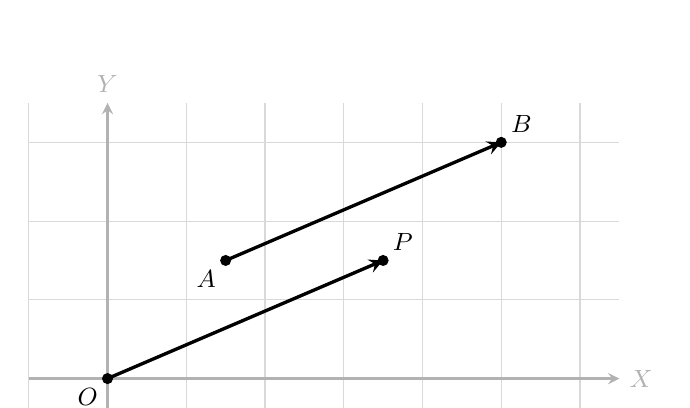
\begin{tikzpicture}[>=stealth, scale=1.0, font=\small]
  % Light background grid
  \draw[gray!30, thin, step=1] (-1, -0.5) grid (6.5, 3.5);
  \draw[->, thick, gray!60] (-1, 0) -- (6.5, 0) node[right] {$X$};
  \draw[->, thick, gray!60] (0, -0.5) -- (0, 3.5) node[above] {$Y$};

  % Vector OP
  \coordinate (O) at (0, 0);
  \coordinate (P) at (3.5, 1.5);
  \draw[->, very thick] (O) -- (P);
  \fill (O) circle (2pt) node[below left] {$O$};
  \fill (P) circle (2pt) node[above right] {$P$};

  % Translated Vector AB
  \coordinate (A) at (1.5, 1.5);
  \coordinate (B) at (5.0, 3.0);
  \draw[->, very thick] (A) -- (B);
  \fill (A) circle (2pt) node[below left] {$A$};
  \fill (B) circle (2pt) node[above right] {$B$};
\end{tikzpicture}
\caption{向量之平移等價性}
\label{fig:b3-fig1-7}
\end{figure}

$\vec{AB}$ 與 $\vec{OP}$ 雖然作為有向線段來說顯然是不同的兩個東西，但看成向量，我們就不加以區分，也就是說，作為向量來看，$\vec{AB}$ 與 $\vec{OP}$ 是代表同一向量，這個道理是因為我們考慮向量時，只考慮一個如下的口令“朝哪個方向前進多遠”而不計較起點，一個向量便相當於一個這樣的口令，（執行口令皆是可以不知自己原來身在何處，只要有了羅盤針及距離表便可以照做）.

要使問題經過向量幾何的轉化後能夠用推演處理，便須充實向量間的運算構造，我們將適當引入向量的加、減、係數積、內積（及外積），以後我們可以看到許多問題轉化成向量的問題後如何利用這些運算來推求未知. 很多時候，向量處理要比座標處理優越，但嚴格說來，向量的運算還是奠定在座標成分的實數系運算上，只是較為簡化符號且授予更清晰的幾何意義.

總結一下：

\textbf{座標幾何}\quad 平面（或空間）的點可由其笛卡兒座標來描述. 而笛卡兒座標的成分（平面上有兩個成分，空間中則需三個）不過是實數. 如此利用實數系的代數運算可推演平面上（或空間中）各種已知或未知的事實.

\textbf{向量幾何}\quad 平面（或空間）的點可由向量（的尾端）來描述. 所有向量自成一個可運算的代數體系（這代數體系中的特別構造如內積（§3-5），外積（第四冊），一方面有它直觀的幾何意義，另一方面又可表成諸向量的座標成分，利用實數系的運算來表示），這代數體系提供了處理與推演的大好場地.

\subsection*{習題 1-2}

\begin{enumerate}[label=\arabic*., leftmargin=2em]
  \item 通常圍棋盤兩邊各 19 目（也就是 18 方格，棋子放在「目」即交點上）. 假想有一棋局正在進行，試給一座標系，以座標描述其第一手到第六手.
  \item 國中物理課講力與運動時就介紹了力的合成與分解試把力的要素及其運算等有關的觀念用圖表示.
\end{enumerate}

\subsection{代數工具的複習提要}
\label{subsec:b3-1-3}

在一、二冊中我們已很辛苦地完成了實數系的建構，練習並瞭解了實數間的運算及性質.

另一方面，世間各種現象常以函數的形式出現，簡單的像
\begin{enumerate}[label=(\arabic*), leftmargin=2em]
  \item 華氏與攝氏溫度的換算：
  \[ y = \frac{9}{5}x + 32 \]
  其中 $x$ 表攝氏度數，$y$ 表華氏度數.
  \item 質點的等速直線運動：
  \[ y = vx \]
  其中 $x$ 表時間，$y$ 為位移，$v$ 為速度，皆為一次函數.
\end{enumerate}

稍複雜的像彈道，便以二次函數來描述，然後我們考慮過一般高次多項式函數：
\[ y = a_0 x^n + a_1 x^{n-1} + \dots + a_{n-1} x + a_n \quad (a_0 \ne 0) \]
更考慮過有理函數，即兩多項式之商，我們知道這些函數間如何運算，也知道所相應的一次方程，二次方程，甚至聯立方程，如何求解.

進一步，為了把乘法變成加法，使計算尺能計算乘法，除法，我們引進來對數函數 $\log_a$，知有
\[ \log_a (uv) = \log_a u + \log_a v;\quad 1 \ne a > 0 \text{ 而 } u, v > 0 \]
對數函數的反函數，則為指數函數.

我們將在第二章中再以三角測量為問題核心，引入三角函數.

這樣，我們大體完備了所需要的函數.（在進一步的數學課程裏，由於極限觀念的大量運用，我們將以“逼近”，探討表為更複雜的函數之自然或人文現象.）

以後各章中，我們將按本章所述處理實際問題的原則，剖析座標幾何、向量幾何的轉化過程，使同學能把實際問題（經由幾何）化成代數問題，而利用我們所學的代數工具去推演有用有利於社會發展的各種結論.

\subsection*{習題 1-3}

\begin{enumerate}[label=\arabic*., leftmargin=2em]
  \item 試將高一所學過的各個代數體系，如自然數系，整數系有理數系實數系的基本運算，即加法與乘法個別整理出來.
  \item 將力的合成與實數的加法所各具有的性質做一比較.
  \item 將計算尺原理做一大略說明（複習第二冊第五章）.
\end{enumerate}


\end{document}
